\documentclass[12pt]{article}

\usepackage[top=3.5cm,bottom=1.5cm,right=3cm,left=3cm]{geometry}
\usepackage{amsthm,amstext,amsmath,amssymb,amsfonts,bbm}
\usepackage{graphicx,bbold,extarrows,multirow,setspace}
\usepackage{epsfig,subfigure,authblk,braket,mathtools}
\usepackage{dsfont,psfrag,stmaryrd,color}
\usepackage[utf8,latin1]{inputenc}
\usepackage[symbol]{footmisc}
\usepackage[x11names,table]{xcolor}
\usepackage{tikz}
\usepackage{hyperref}
\hypersetup{
    hypertexnames=true,
    colorlinks=true,  
    filebordercolor=red,
    linkcolor=red, 
    urlcolor=olive,
    citecolor=orange,
    pdftitle={A first look into Quantum Logic},
    pdfauthor={A. Haddad}}
\usepackage{cite}
\usepackage[backend=biber,style=numeric,bibencoding=utf8]{biblatex}
\addbibresource{biblio.bib} 
\usepackage{footmisc}
%{\footnotesize\bibliography{bibfile}}

\providecommand{\keywords}[1]
{
  \small	
  \textbf{\textit{Keywords :}} #1
}

\begin{document}
%%%%%%%%%%%%%%%%%%%%%%%%%%%%%%%%%%%%%%%%%%%%%%%%%%%%%%%%%%%%%%%%%%%%%%%%%%%%%%%%%%%
\begin{titlepage}
\title{\Huge{\textbf{A first look into Quantum Logic}}}
\author{{\large{A. Haddad}}\thanks{\href{mailto:abdelhamid.haddad@etu.univ-amu.fr}{abdelhamid.haddad@etu.univ-amu.fr}}}
\affil{\Large Aix-Marseille University, Marseille, France.}
\maketitle
\thispagestyle{empty}
\centering
\large Work presented to complete the scientific watch course \\	
\large Supervised by: \textbf{T.Krajewski}\footnote[2]{\thanks{\href{mailto:thomas.krajewski@cpt.univ-mrs.fr}{thomas.krajewski@cpt.univ-mrs.fr}}}
\vspace{2cm}
\begin{abstract}
\normalsize
\begin{spacing}{1.2}
In an attempt to give an overview on \textit{"Quantum logic"}. We present some abstract mathematical notions to be self-consistent as possible and show how they are structured to form a \textit{"Classical logic"} which in fact is a \textit{Boolean structure}, we'll see how relaxing the distributive property is needed to define what seems to be a "Quantum logic". Then, in a sort of a bottom-up approach we will try to reconstruct our habitual Quantum mechanics, passing through Hilbert spaces $\mathcal{H}$, Plank's constant $\hbar$ and bell's inequalities among other things.
\end{spacing}
\end{abstract}
\keywords{Classical \& Quantum logic, Quantum Foundations, orthomodular lattice, Hilbert lattice, Planck's constant, Bell's inequalities.}
\end{titlepage}
%%%%%%%%%%%%%%%%%%%%%%%%%%%%%%%%%%%%%%%%%%%%%%%%%%%%%%%%%%%%%%%%%%%%%%%%%%%%%%%%%%%
\clearpage
\renewcommand{\thefootnote}{\arabic{footnote}}
\newgeometry{top=1.5cm,bottom=2cm,right=1.5cm,left=1.5cm}
\setstretch{1.3}
\setcounter{page}{2}
%%%%%%%%%%%%%%%%%%%%%%%%%%%%%%%%%%%%%%%%%%%%%%%%%%%%%%%%%%%%%%%%%%%%%%%%%%%%%%%%%%%
\section{Introduction and Motivation(s)}

Among many great revolutions associated to the merging of Quantum Mechanic (QM) all over the 20th century, some of them have been largely understood and found many applications suck as Electronic Microscopy (1931) and Nuclear Magnetic Resonance (NMR, in 1938), other ones was more conceptual such as wave-particle duality (1924), Heisenberg uncertainties (1927) and bell's inequalities (1964), but some of them are more surprising, right ? like Teleportation (1993) or Entanglement (1935)\footnote{More complete discussions can be found in \cite{manjit, omnes}.\label{footref}}

\vspace{0.3cm}
Paying attention to the large period between theses events which seems pretty long (almost a century), was it because physicist mind (and humanity) wasn't ready to absorb such and ideas or it was a lack of clarity in the formalism used to express QM itself ? The idea is to think that it may exist a more adequate formalism to express some Quantum foundations and one of them :\textit{"Quantum Logic"} (QL).

\vspace{0.3cm}
We haven't the pretension to say that we are a precursor to this, firstly initiated in the milestone paper \cite{Birkhoff}, a lot of physicist revisit this subject and redefine it more properly\footref{footref}. Starting by some logical preliminary tools applied to Classical mechanics (CM) first then in QM, gives some important remarks on the validity of such an approach, briefly aboard Plank's constant and Bell's inequalities in QL. We conclude discussing some future approach such as fuzzy QL and Non-commutative QL.

\vspace{-0.3cm}
\section{Logic and Physics}
\vspace{-0.2cm}

Maybe some of you when reading this kind of topic for the first time ask themselves (as me for the first time) \textit{"What the hell will connects physics to logic ?"}

A simple answer would be : \textit{Logic is the science that studies thinking.} but the answer is not so simple and you may consult \cite{fuzzy3,logic} for more details. We will focus on some physical explanations and try to let it more intuitive. We will follow \cite{fuzzy3,david,isham,mackey,one,two} in this section.

\vspace{-0.4cm}
\subsection{Preliminaries}

Without going much into the details, all that will follow is related to the notion of a \textit{"Lattice"} $\mathcal{L}$. Personally, it took me a long time to understand it, but it became clearer knowing that the name \textit{lattice} is suggested by the form of the \textbf{Hasse diagram} that depicting it as shown in fig.\ref{lattice}. we will highlight some important concepts following \cite{david,fuzzy3,pavicic1999non}. 

\begin{figure}[ht!]
\centering
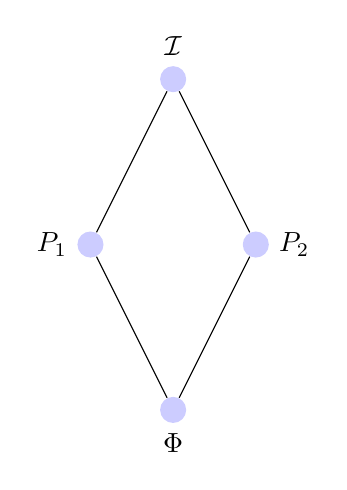
\begin{tikzpicture}[scale=.7,
    mycirc/.style={circle,fill=blue!20, minimum size=0.3cm}
    ]
    \node[mycirc,label=left:{$P_1$}] (n1) at (0,0) {};
    \node[mycirc,label=right:{$P_2$}] (n2) at (3,0) {};
    \node[mycirc,label=above:{$\mathcal{I}$}] (n3) at (1.5,3) {};
    \node[mycirc,label=below:{$\Phi$}] (n4) at (1.5,-3) {};
    \draw (n1) -- (n3) -- (n2) -- (n4) -- (n1);
\end{tikzpicture}

\caption{{\footnotesize "Simple" Hasse diagram of a \underline{partially ordered} from bottom to top \underline{bounded} by the least or \textit{"absurd proposition"} \textbf{$\Phi$} (0) and the greatest or \textit{"Sure proposition"} \textbf{$\mathcal{I}$} (1) \underline{lattice} ($\mathcal{L}$,$\leq$,$\land$,$\lor$,0,1) with random propositions $P_1$ and $P_2$ in each vertex.}}\label{lattice}
\end{figure}

\begin{itshape}
\textbf{First.} A lattice $\mathcal{L}$ is a set of elements (propositions), partially ordered $\leq$, with a greatest lower bound (meet or infimum) $x~\land ~y$ and a least upper bound (join or supremum) $x~\lor ~y$: ($\mathcal{L}$,$\leq$,$\land$,$\lor$).

\textbf{Second.} A bounded lattice have a least and a greatest elements $0~\leq~1$ ($\mathcal{L}$,$\leq$,$\land$,$\lor$,0,1), will be denoted as $\mathfrak{L}$.

\textbf{Third.} If $x,x'~\in~\mathfrak{L}$ satisfies $x~\land~x'~=~1$ and $x~\lor~x'~=~0$, then $x'$ is called the complement of $x$. If in addition, $\forall x~\in~\mathfrak{L}$ has a unique complement, the lattice is said to be uniquely complemented.

\textbf{Fourth.} A lattice $L=$($\mathcal{L}$,$\leq$,$\land$,$\lor$) is modular iff: 
$$x~\leq~y~\Rightarrow~x\land(z \lor y)~=~(x \land z)\lor y,~\forall z \in L$$.

If $\mathfrak{L}$ satisfies the same relation, it will be called an \textit{"orthocomplemented lattice"} (OcL).

\textbf{Fifth.} An OcL $\mathfrak{L}$ is called \textit{Boolean} if it satisfies: (distributivity) 
\begin{equation}
x\land(y \lor z)~=~(x \land y)\lor(x \land z).\label{equiv}
\end{equation}
\end{itshape}
\vspace{-0.9cm}
\subsection{Classical}

In fact, any physical theory are based on some axioms and theorems given in a form of \textit{sentences} first, then by a hole program of formalization\footnote{The problem of formalization of simple mathematical theories has been solved by the concept of a \textit{first-order theory.}\cite{1}}, they will be compiled and the outcomes will be a full viable physical theory. Then, the logical "game" will be to understand the structure behind these sentences and how they are connected by means of some logical connectives.

To explain the meaning of these terms, we must appeal to the well-known \textit{Newtonian mechanics} where one of their best realisation is in the Hamiltonian formulation : For a system with n degrees of freedom, a state is a point x in the 2n dimensional phase space $\Omega$.

A system can then be associated to some specific properties such as having a certain position (or in an interval $\delta$), a momentum or energy, if it is a proton or an electron or whatever you want ! All this will be nicely captured as seen as a \textit{set of propositions}, that can be verified to be \textit{TRUE} or \textit{FALSE} with a certain (logical) structure.

It follows from this arrangement of propositions that the corresponding logic is identical to that of some Boolean algebra of subsets of the state space $\Omega$, and from last section, If $\mathcal{L}$ is a Boolean algebra, than $\mathcal{L}$ is modular, orthomodular and orthocomplemented. Which resume our developments in the logical mathematical structure of classical physics.

\vspace{-0.4cm}
\subsection{Quantum}

Now, the novelty arise when dealing with the principles of QM where quantities such the position and momentum are promoted to operators know as \textit{"observables"}\footnote{Where in classical mechanics, there was no need to differentiate between the state of the system and observables.} and are characterized by the fact that conjugate pairs cannot be simultaneously measured, also known as \textit{"Heisenberg's Uncertainty Principle"} as shown in fig.\ref{fig1}.

\begin{figure}[ht!]
\centering
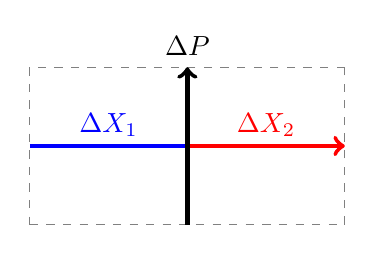
\begin{tikzpicture}
\draw[-,gray,dashed] (-1,1)--(3,1);
\draw[-,gray,dashed] (3,1)--(3,3);
\draw[-,gray,dashed] (3,3)--(-1,3);
\draw[-,gray,dashed] (-1,3)--(-1,1);
\draw[->,red,ultra thick] (1,2)--(3,2);
\draw[-,blue,ultra thick] (-1,2)--(1,2);
\draw[->,ultra thick] (1,1)--(1,3) node[above]{$\Delta P$};
\draw (0,2) node[text=blue,above]{$\Delta X_1$};
\draw (2,2) node[text=red, above]{$\Delta X_2$};
\end{tikzpicture}

\caption{{\footnotesize Schematic representation to illustrate how the distributive law fails in QM, consider the rectangle represent the allowed regions by Heisenberg uncertainties and three propositions: P1: The particle has momentum in $\Delta P$, P2: The particle is in $\Delta X_1$, P3: The particle is in $\Delta X_2$. We observe for example that the left hand side of the first equation in \eqref{equiv} is "TRUE" but the right hand side are both "FALSE" ! Since they assert tighter restrictions on simultaneous values of position and momentum than is allowed by QM.}}\label{fig1}
\end{figure}

Then the point is that the sets of properties (developed above) of classical and quantum systems have an OcL structure both, but differs into their distributivity or not ! 

The starting point of all that was in \cite{Birkhoff} when propositions (observables) was associated to projection operators \textbf{$\hat{P}$} which will be "TRUE" if the vector $|\Psi>$ is an eigenvector of \textbf{$\hat{P}$} (and inversely). As \textbf{$\hat{P}$}'s are associated to closed subspace of $\mathcal{H}$, by analogy: propositions are associated to such subspace which satisfied all what we've said earlier and define the so-called \textit{Hilbert lattice}, this was nicely developed in \cite{david}.


\vspace{-0.3cm}
\section{Is "Quantum logic" a valid theory ?}
\vspace{-0.2cm}

It was surprising when preparing theses notes to find in \cite{pavicic1999non}\footnote{Unfortunately, we found this work a bit late but we judged important to cite.} that QL can also be modeled as a \textit{weakly orthomodular lattice} and that CL is also modeled by a \textit{weakly distributive lattice}, and both new models turn out to be non-orthomodular lattices. 

But even with this, we will present two milestone notions of QM from the point of view of QL (the OcL !), namely: the \textit{Plank's constant} and \textit{Bell's inequalities}.

%\vspace{-0.4cm}
\subsection*{Plank's constant}

QM is mostly associated with the (reduced) Planck's constant $\hbar$, it is often natural to think that it should appear somewhere in any formulation, right ? This subsection will be mostly based on \cite{plank} which we highly recommend you to read !

Planck's constant is widely considered as a characteristic of QM that indicates the border line between the quantum and classical worlds, and the QL sketched above doesn't contain the necessary tools to describe classical realm since it appears as an abstract and empty theory (remind that we have obtained it by relaxing classical logic) and then there is no hope to find any $\hbar$.

Dealing with some classical concepts of \textit{localizability} and \textit{homogeneity} in order to define the notion of \textit{particles} and their movement of a point in the configuration space (which should be invariant under Galileo transformations), the author \cite{plank} was able to link all that it to our $\hbar$ and said : 

\begin{quote}
\textit{Hence, our first, still preliminary result is, that for discovering the physical meaning of
Planck's constant $\hbar$, in addition to the abstract QL, classical concepts must be taken into account. However, this result would invalidate the idea of an autonomous quantum world without any recourse to a classical world.}
\end{quote}

We should also remark that there was an attempt from the same author who in \cite{relativistic} have tried to develop a \textit{Relativistic QL}.

\vspace{-0.4cm}
\subsection*{Bell inequalities}

\textit{Entanglement} was one of the most discussed\footref{footref} features of QM, he led to the emergence of the so-called \textit{EPR paradox} which claim that: 1) QM is incomplete or 2) QM is non-local. EPR suppose the existence of some \textit{local hidden variables} (HV) in QM. Bell's inequalities was the culminate point to solve this paradox asserting that a HV theory should satisfies: 

\begin{equation}
|P(A,B)~-~P(A,C)|~\leq~1~+~P(B,C).\label{bell}
\end{equation}  

where P stands for probability and A,B,C are some random variables taking only the values $\pm 1$.

It is interesting to see how all this have been studied using the tools of quantum logic as discussed in \cite{bell1,bell2,bell3}, we highlighted based on \cite{bell2} the essential argument :   


For any two proposition A,B in a lattice $\mathcal{L}$, we define a (pseudo)metric such that: 

\begin{equation}\begin{aligned}
&d(A,B)~=~P(A \lor B)~-~P(A \land B),\\ 
&0~\leq~d(A,B)~\leq~1~,~d(A,A)~=~0.\label{metric}
\end{aligned}\end{equation}

Satisfying the following triangle inequality which are closely related to Bell inequalities \eqref{bell} (see \cite{santos}): 

\begin{equation}
|d(A,B)~-~d(A,C)|~\leq~d(B,C)~\leq~d(A,B)~+~d(A,C).\label{final}
\end{equation}

The point is, if we consider a Boolean structure (CM), the inequality \eqref{final} hold true\footnote{Unfortunately, we haven't found a complete proof of it but we will trust our peers, at least for the moment.}, but a non-Boolean structure (QM) this will break the inequality\footnote{The explanation is if two of the observables, say A and B, are not compatible then their distance is not defined because QM does not provide a joint probability of two incompatible observables.} as QM do with Bell's inequalities.  

\vspace{-0.4cm}
\section{Conclusions}
\vspace{-0.2cm}

Surely, our presentation is incomplete and the goal was neither to be complete nor to be original, and there is a lot who have been left to other occasions. We summarized here our most important conclusions:
 
\begin{itemize}
\item The sets of properties of classical and quantum systems have both an OcL structure.
\item The distributive property provides the essential difference between classical and quantum theories. 
\item We can extract a Planck's constant $\hbar$ in QL but we should take account of classical concepts (\textit{localizability} and \textit{homogeneity}).
\item QL may provide an equivalent inequalities to the well-know "Bell's inequalities" which increase our trust on QL formulation.
\end{itemize}

We also present some related research fields and maybe future directions:

\begin{itemize}
\item \textbf{Fuzzy logic :} As shown, quantum logic seems as a particular case of classical one. The point is there exist different "sort" of logic as \textit{fuzzy logic} where a proposition in not just "TRUE" or "FALSE" but can take values in the whole interval [0,1]\footnote{This is helpful to treats ambiguities on propositions that cannot be stated to be "TRUE" or "FALSE".}. Many works have been done to generalize quantum logic to fuzzy quantum logic, especially in \cite{fuzzy3,pavicic2009quantum,pykacz1987quantum,pykacz1994fuzzy}.
\item \textbf{Non-Commutative Geometry (NCG) :} Coincidentally, as for a QM system can be represented as an OcL, there exist an algebraic setting, namely the $W^*$-algebra where the set of projectors of any $W^*$-algebra has the same structure of an OcL ! Therefore it has been proposed to be identified as a model for the propositional lattice of physical systems, and as the $W^*$-algebra depend on $\hbar$, they characterize both quantum and classical ($\hbar~=~0$) systems. The story continue if we imagine a Non-commutative $W^*$-algebra. All this and more will be found in \cite{marchetti2007quantum} and references therein.
\end{itemize}

\vspace{-1cm}
\section*{Acknowledgements}
\vspace{-0.2cm}

The author warmly acknowledge Pr. T. KRAJEWSKI (Aix Marseille Univ, Universit\'e de Toulon, CNRS, CPT, Marseille, France) for guiding advises and inspiring mentoring throughout this work, and also their classmates A. HARIFENO and N. ROCQUELAIN for various discussions during our sessions.

\vspace{0.5cm}
\begin{small}
\vspace{-0.2cm}
{\setstretch{1.0}
\fontsize{2pt}{0.2cm}\selectfont
\printbibliography}
\end{small}
\end{document}
